\documentclass[11pt]{article}

\usepackage[utf8]{inputenc}
\usepackage{graphicx}
\usepackage{geometry}
%\geometry{a4paper, margin=1in} % Adjust margins as needed
\usepackage{hyperref} % For clickable URLs
\usepackage{caption} % For customizing captions
\usepackage{booktabs} % For better tables (optional)
\usepackage{enumitem} % For customizing lists (optional)

% For math
\usepackage{amsmath}
\usepackage{amsfonts}
\usepackage{amssymb}

% For algorithms
\usepackage{algorithm}
\usepackage{algpseudocode}

% For citations
\usepackage{natbib}  

% For images
%\usepackage{float}

% Define some colors (optional)
%\usepackage{xcolor}
%\definecolor{darkblue}{rgb}{0,0,0.5}

% Set up title and author information
\title{Social Media Course Project \\ [1em] \Large Application of Transformer-Like Deep Neural Network Architecture For Graph Edge Prediction}
%\title{Encoder-Like Deep Neural Network Architecture For Graph Edge Prediction}
\author{Bruno Guzzo \\ 242504}
\date{Winter 2025}

% Customization for captions
\captionsetup[figure]{labelfont=bf, font=small, justification=centering, labelformat=empty, labelsep=period} % Customize as needed
\captionsetup[table]{labelfont=bf, font=small, justification=centering, labelformat=empty, labelsep=period} % Customize as needed


\begin{document}
	
	\maketitle
	
	\begin{abstract}
	This project explores the application of transformer-like Graph Neural Networks (GNNs) for edge prediction in semantic graph. The project aims to demonstrate the effectiveness of GNNs with architectural features inspired by transformer networks in capturing complex relationships and predicting potential connections within a graph dataset.
	\end{abstract}
	
	
	\section{Introduction}
	The main given guideline assignment for the present project is \textit{"Application of GNN on semantic graph generated by LLMs"}. To address such abstract assignment we chose a \textit{"homemade"} approach in which we build from scratch a dataset and a neural network to solve the assignment. \\
	Our baseline idea is to build a dataset of graphs form Wikipedia article links where each node is a page title, then design a custom neural network to operate on such data type.\\
	To design such custom neural network we get inspired by the latest development in natural language processing and graph neural network. \\
	Thus, we adopt a deep neural network architecture that extend the encoder stack of the transformer \cite{vaswani2023attentionneed} with the application of graph attention network \cite{veličković2018graphattentionnetworks}.
	
	
	\section{Literature Review: Graph Attention}
	\label{graph_attention}
	Graph Attention Networks (GATs) are a class of neural network architectures designed to operate on graph-structured data. They leverage a self-attention mechanism \cite{vaswani2023attentionneed} to dynamically learn the importance of neighboring nodes, enabling effective feature aggregation while being independent of the underlying graph structure and allowing inductive learning.
	
	\subsubsection{Graph Attention Layer}
	The fundamental building block of a GAT \cite{veličković2018graphattentionnetworks} is the \textit{graph attentional layer}. Given a graph with $N$ nodes, each represented by a feature vector $\mathbf{h}_i \in \mathbb{R}^F$ ($i \in \{1, \dots, N\}$), the objective is to produce a new set of node features, $\mathbf{h}_i' \in \mathbb{R}^{F'}$.
	
	\subsubsection{Feature Transformation}
	Initially, each node's feature vector is linearly transformed:
	\begin{equation}
		\hat{\mathbf{h}}_i = \mathbf{W} \mathbf{h}_i,
	\end{equation}
	where $\mathbf{W} \in \mathbb{R}^{F' \times F}$ is a learnable weight matrix.
	
	\subsubsection{Attention Mechanism}
	Next, an attention mechanism is employed to compute the importance of node $j$'s features to node $i$. This is achieved through a shared attentional mechanism $a: \mathbb{R}^{F'} \times \mathbb{R}^{F'} \rightarrow \mathbb{R}$:
	\begin{equation}
		e_{ij} = a(\hat{\mathbf{h}}_i, \hat{\mathbf{h}}_j).
	\end{equation}
	In practice, $a$ is often implemented as a single-layer feed-forward neural network with parameters $\mathbf{a} \in \mathbb{R}^{2F'}$:
	\begin{equation}
		e_{ij} = \text{LeakyReLU}\left( \mathbf{a}^T [\hat{\mathbf{h}}_i || \hat{\mathbf{h}}_j] \right),
	\end{equation}
	where $||$ denotes concatenation and $\text{LeakyReLU}$ is a nonlinear activation function.
	
	\subsubsection{Masked Attention}
	To incorporate graph structure, the attention mechanism is masked. The coefficients $e_{ij}$ are only computed for nodes $j \in \mathcal{N}_i$, where $\mathcal{N}_i$ is the set of neighbors of node $i$ (including $i$ itself).
	
	\subsubsection{Normalization}
	The coefficients are then normalized using a softmax function over the neighborhood of each node:
	\begin{equation}
		\alpha_{ij} = \frac{\exp(e_{ij})}{\sum_{k \in \mathcal{N}_i} \exp(e_{ik})}.
	\end{equation}
	
	\subsubsection{Feature Aggregation}
	Finally, the new feature vector for node $i$ is calculated by aggregating the transformed features of its neighbors, weighted by the normalized attention coefficients:
	\begin{equation}
		\mathbf{h}'_i = \sigma \left( \sum_{j \in \mathcal{N}_i} \alpha_{ij} \hat{\mathbf{h}}_j \right),
	\end{equation}
	where $\sigma$ is a nonlinear activation function.
	
	\subsubsection{Multi-Head Attention}
	To stabilize the learning process and capture different aspects of node relationships, multi-head attention is utilized.  The operation of the graph attention layer is performed $K$ times in parallel, each with a separate transformation and attention parameters $\mathbf{W}^k$ and $\mathbf{a}^k$ (respectively). The output of each head is a new node feature vector, $\mathbf{h}_i^{'k}$.
	
	\subsubsection{Concatenation}
	The output from the different heads can be concatenated together:
	\begin{equation}
		\mathbf{h}'_i = \underset{k=1}{\overset{K}{\parallel}} \sigma \left( \sum_{j \in \mathcal{N}_i} \alpha_{ij}^k \mathbf{\hat{h}}_j^k \right).
	\end{equation}
	In this case, the final output feature vector will have the dimension $KF'$.
	
	\subsubsection{Averaging}
	Alternatively, for the final layers, the outputs can be averaged followed by the final activation:
	\begin{equation}
		\mathbf{h}'_i = \sigma\left(\frac{1}{K} \sum_{k=1}^K \left( \sum_{j \in \mathcal{N}_i} \alpha_{ij}^k \mathbf{\hat{h}}_j^k \right) \right).
	\end{equation}
	Here, the final output feature vector has the dimension $F'$.

	\section{Wikipedia Articles Link Dataset}
	Given the necessity of a consistent graph dataset to train our GNN we chose to build a suited dataset to address the project needs.
	Each data point of our dataset is a graph where each node is a Wikipedia article title and the edges represent links between them. The presence of an edge $(u, v)$ means that the article $u$ cite article $v$ in its body or vice-versa.
	Following this principle we obtain a non-directed graph where the edges indicate that two articles are somehow related.
	\begin{figure}[h] % h! means "here" and try hard
		\centering
		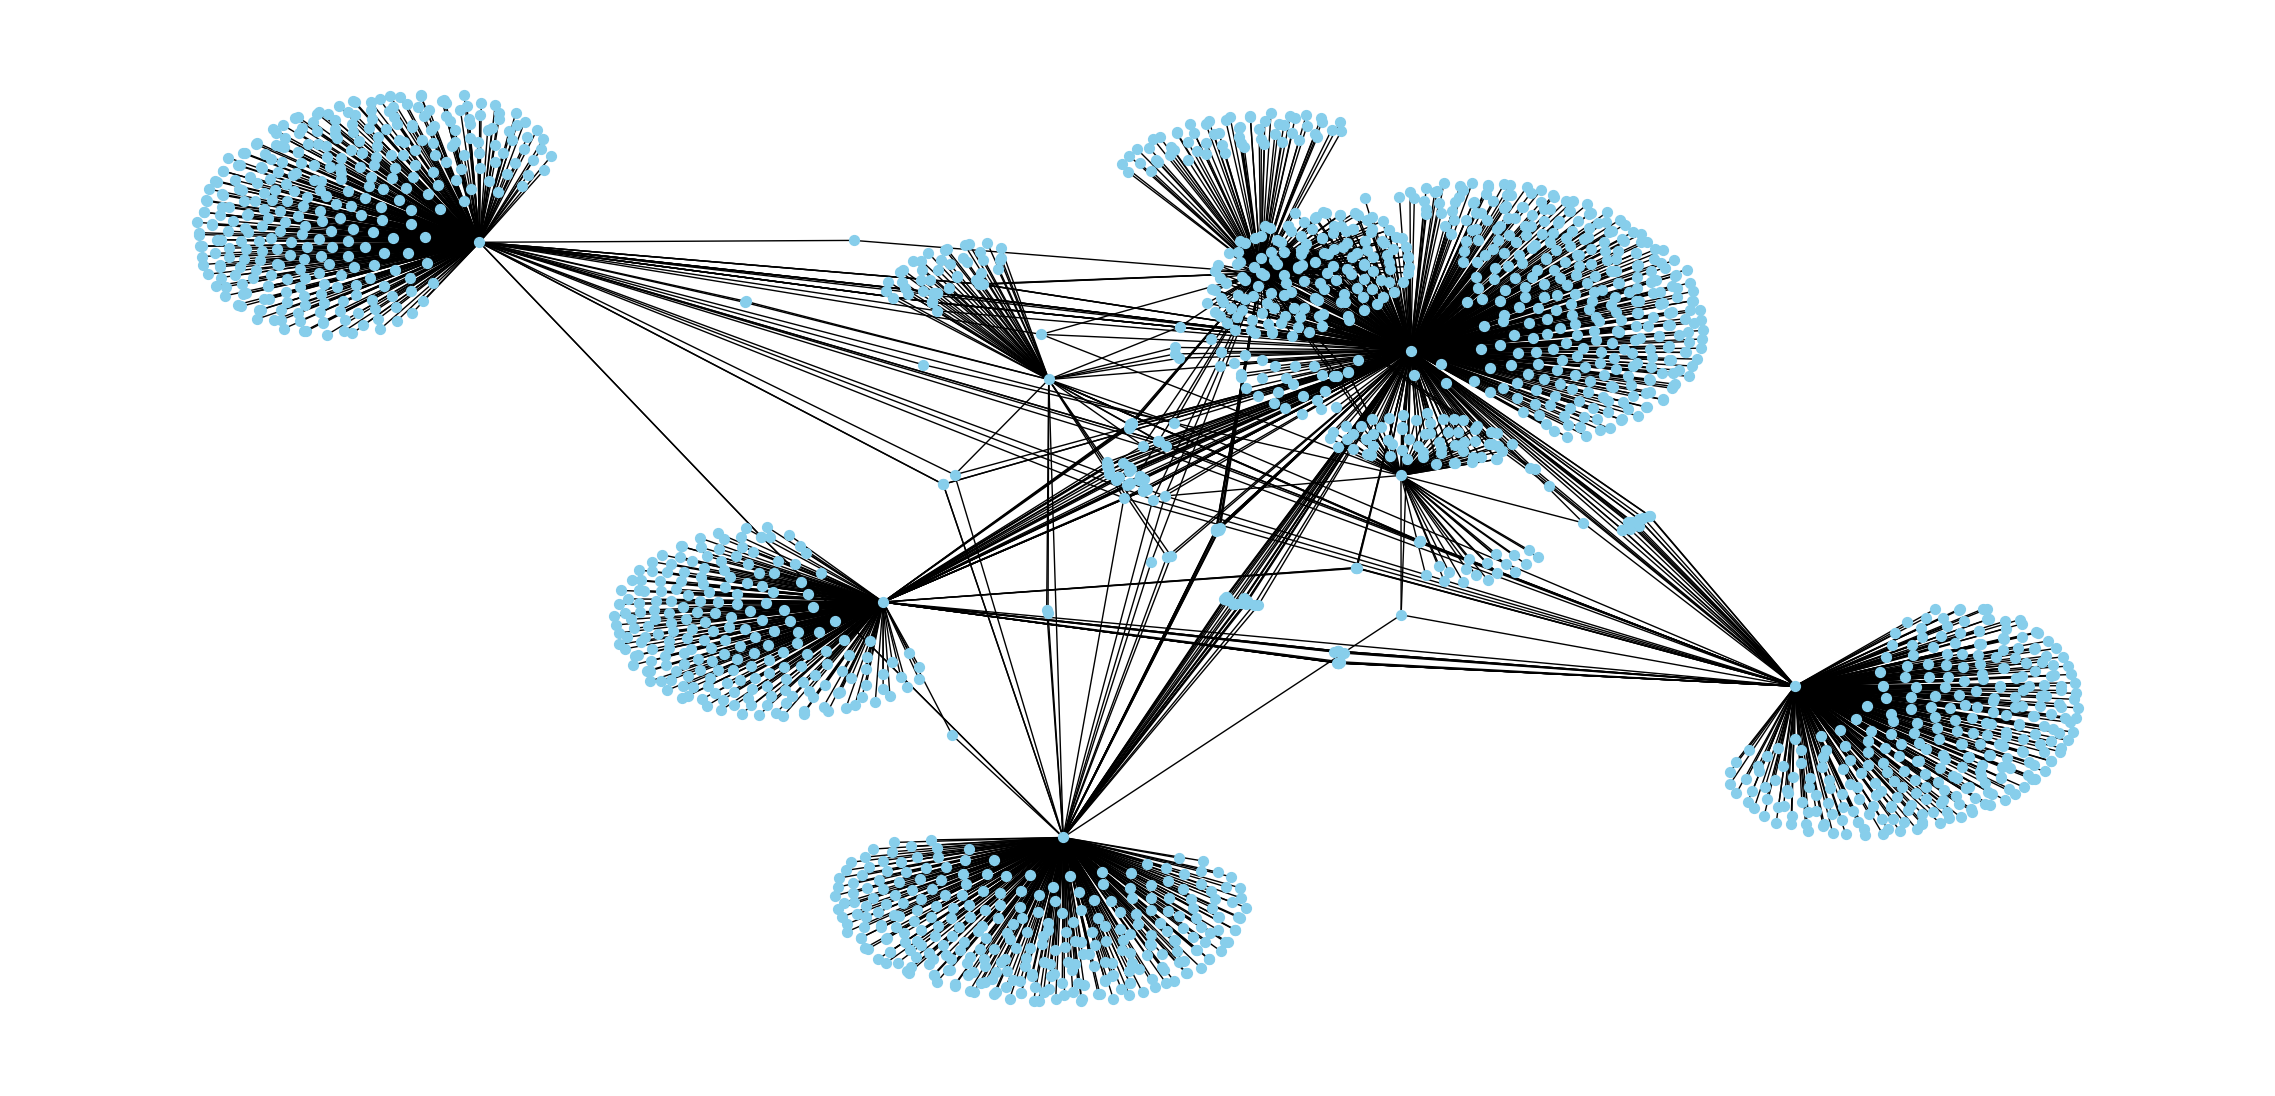
\includegraphics[width=1\textwidth]{images/wiki_link_grap_2k.png}
		\caption{Figure 1: A graph of 2000 nodes built form the root article title 'Sustainability'.}
	\end{figure}
	
	\subsection{Graph Extraction Algorithm}
	To obtain the graphs of our dataset we adopt a \textbf{breadth first strategy} to explore Wikipedia article links starting for a \textbf{root article}. This prioritize the inclusion of the immediate neighborhood of the root article.
	We adopt this methodology against a \textbf{depth first strategy} so we can have all the immediate neighbors of the root node, thus leading to a \textbf{robust representation} of the root article.
	This is particular helpful when using GNN where the network learn a node representation using the information present in it's first neighbors.\\\\
	The final graph produced by our algorithm is limited by a maximum size of \textbf{20000 nodes}. This allow us to obtain a graph that capture the deep structure of Wikipedia. \\
	Below we present a simplified \textbf{pseudo-code} of the BFS algorithm used, the final version is \textbf{recursive} and have several constraint to enforce graph consistency. 
	
	\begin{algorithm}
		\caption{Wikipedia Graph Extraction using BFS}
		\begin{algorithmic}[1]
			\Require $rootArticleTitle$, $maxNodes$
			\State $graph \gets$ new Graph
			\State $visited \gets$ new Set, initialized with $rootArticleTitle$
			\State $queue \gets$ new Queue, enqueue $rootArticleTitle$
			\State $graph$.addNode($rootArticleTitle$)
			\While {$queue$ is not empty and $|graph.nodes| < maxNodes$}
			\State $pageTitle \gets queue$.dequeue()
			\State $page \gets$ getWikipediaPage($pageTitle$) \Comment{Handles Page/Disambiguation Errors}
			\If {$page$ is not valid}
			\State \textbf{continue} \Comment{Skip to the next page in queue}
			\EndIf
			\For {$linkTitle$ in $page.links$}
			\If {$|graph.nodes| \geq maxNodes$}
			\State \textbf{break} \Comment{Exit loop}
			\EndIf
			\If {$linkTitle \in visited$}
			\State $graph$.addEdge($pageTitle$, $linkTitle$)
			\Else
			\State $visited$.add($linkTitle$)
			\State $queue$.enqueue($linkTitle$)
			\State $graph$.addNode($linkTitle$)
			\State $graph$.addEdge($pageTitle$, $linkTitle$)
			\EndIf
			\EndFor
			\EndWhile
			\If {not isConnected($graph$)}
			\State \textbf{Error:} Graph is not connected
			\EndIf
			\State \textbf{return} $graph$
		\end{algorithmic}
		\label{alg_1}
	\end{algorithm}
	
	\subsection{Node Embedding}
	\label{node_embedding}
	To efficiently use our dataset with GNN it is needed to \textbf{embed each node} in way that it can be processed in a numerical way. To do so, we relay on state-of-the-art sentence embedding model to transform node labels in numeral representation.
	We chose to use a freely and open-source available \textbf{sentence-transformers} model: \textbf{\href{https://huggingface.co/sentence-transformers/all-MiniLM-L6-v2}{all-MiniLM-L6-v2}} \cite{reimers-2019-sentence-bert}. \\\\
	It maps sentences and paragraphs to a \textbf{384 dimensional dense vector space} and can be used for tasks like \textbf{clustering} or \textbf{semantic search}.
	\textbf{all-MiniLM-L6-v2} is derived from the MiniLM \cite{wang2020minilmdeepselfattentiondistillation} architecture and it leverages a distilled version of the \textbf{BERT} (Bidirectional Encoder Representations from Transformers) \cite{devlin2019bertpretrainingdeepbidirectional} model.\\
	The description of this model is outside the scope of this project and it is already been exposed in our previous natural language processing project.,
	
	\subsection{Final Dataset}
	The final dataset has been generated by executing the \textbf{algorithm \ref{alg_1}} on a list of Wikipedia article titles and saving the graph information (nodes and edges) in JSON files.
	We used a list of Wikipedia article titles related to \textbf{sustainability and development} (around $300$), but we have also included the \textbf{top 50 most visited} article in 2024.
	This would ensure that the final GNN model will preserve a small but broad \textbf{generalization capability}.\\\\
	However, to ensure fast data loading, we have also created a \textbf{tensor} file version of the dataset which include node embedding and labels as well.
	Thus, the final dataset is composed of \textbf{389 graphs} with \textbf{20000 nodes each}, this amount to roughly \textbf{7 million of nodes}. It worth it to note that, of course, some graphs could share common node labels.\\
	
	
	\section{Graph Neural Network Architecture}
	Before to get to the final network architecture it is important to remark decisions and ideas that lead us to develop such architecture. 
	\begin{itemize}
		\item{\textbf{Problem complexity}}: The link prediction task is not easy, especially when dealing with thousands of nodes and edges. It is needed to capture relation between distant nodes. So, the propagation of the information form nodes to nodes is crucial to ensure optimal result. For this reason, we could hypnotize the need for a \textbf{deep neural network} to address the long information transfer needed. 
		
		\item{\textbf{Dealing with graphs}}: Each data point of our dataset ia a huge graph, so it is needed to use state-of-the-art graph neural network methodology to deal with such objects. We chose to adopt the aforementioned \textbf{graph attention} \cite{veličković2018graphattentionnetworks} \ref{graph_attention} since it has shown better results than convolutional graph neural network \cite{kipf2017semisupervisedclassificationgraphconvolutional}. 
		
		\item{\textbf{Dealing with words}}: Despite he graphic nature of the problem we are fundamentally trying to learn relation from words and small phrases. This is a common problem of \textbf{NLP} (Natural Language Processing). So, it is natural to look to the solutions applied in such filed to take inspiration from. This intuition lead us to chose a sub-layer structure similar to the one used in the well-known \textbf{transformer architecture} \cite{vaswani2023attentionneed}.   
	\end{itemize}
	
	\subsection{Network Architecture In Detail}
	Our network architecture for link prediction on graph structured data is composed by the \texttt{GatModel} class and it is built around a custom \texttt{DeepGATBlock} module.
	The complete architecture is designed to process graph data, and performs node embeddings, multi-layered graph attention, and link prediction through a dot product decoder.
	
	\begin{figure}[h] % h! means "here" and try hard
		\centering
		\label{figure_2}
		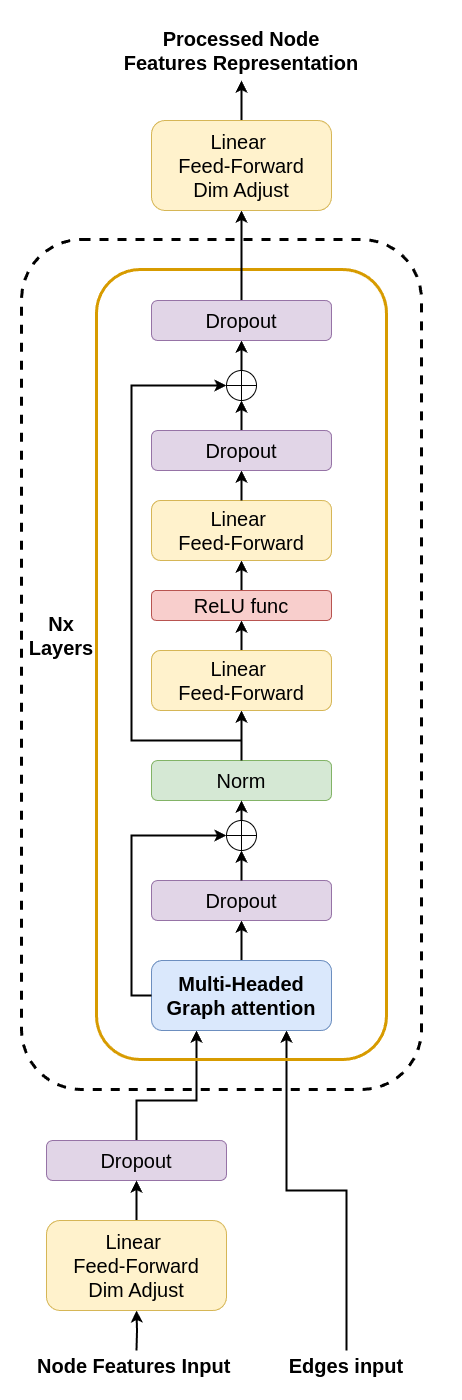
\includegraphics[height=0.8\textwidth]{images/custom_gnn_diagram.png}
		\caption{Figure 2: Graphical representation of the our final \textbf{graph neural network}.}
	\end{figure}
	
	The \texttt{GatModel} model consists of the following components:
	\begin{enumerate}
		\item An input dropout \cite{JMLR:v15:srivastava14a} layer to regularize input features.
		
		\item An input linear layer, $L_{in}$, that projects the input features into the hidden feature space.
		
		\item A \texttt{DeepGATBlock}, which applies multiple levels of GAT layers, dropout, normalization, and Feed-Forward layers, as we will discuss in next section.
		
		\item An output linear layer, $L_{out}$, which transforms the processed hidden features into the final embedding space.
	\end{enumerate}
	
	\subsubsection{Mathematical Representation Of \texttt{GatModel}}
	The \textbf{encoding} process can be mathematically expressed as follows:
	\begin{enumerate}
		\item Given an input node feature matrix $X \in \mathbb{R}^{N \times F_{in}}$, where $N$ is the number of nodes and $F_{in}$ is the number of input features.
	
		\item The input features undergo a linear transformation and dropout:\\ 
		$X' = Dropout(L_{in}(X))$, where $L_{in} : \mathbb{R}^{F_{in}} \to \mathbb{R}^{H}$, and $H$ is the number of hidden channels.
		
		\item The transformed features, $X'$, are processed by the \texttt{DeepGATBlock}:\\ 
		$Z = \text{DeepGATBlock}(X', E)$, where $E$ represents the edge index of the graph.
		
		\item Finally, a linear projection is applied to the GAT block output: $Z_{out} = L_{out}(Z)$, where $L_{out}: \mathbb{R}^H \to \mathbb{R}^{F_{out}}$ and $F_{out}$ is the number of output channels.
	\end{enumerate}
	The \textbf{decoder} then computes the logits of edge existence based on the \textbf{dot product of node embeddings} extracted by the encoder: $\text{logits}_{ij} = (z_i \cdot z_j)$, where $z_i$ and $z_j$ are the embeddings of node $i$ and $j$, respectively.
	
	
	\subsubsection{\texttt{DeepGATBlock} Architecture}
	The \texttt{DeepGATBlock} is a modular block composed of a series of \textit{levels}, each of them processing node embeddings using a combination of graph attention mechanism, feed-forward network and normalization technique.
	Each level consists of the following operations:
	\begin{enumerate}
		\item A \textbf{multi-head graph attention layer}, $GAT$, which attends to the features of neighboring nodes.
		The output of the multi-head attention is not concatenated but rather averaged to match the input dimension.
		Given a node feature matrix $X \in \mathbb{R}^{N \times H}$ and an edge index $E$, the GAT layer calculates node representation according to the Graph Attention mechanism: $X_{att} = GAT(X, E)$, where the result $X_{att}$ is in $\mathbb{R}^{N \times H}$.
		
		\item An attention \textbf{dropout layer} to regularize attention output.
		
		\item A \textbf{residual connection} between input features and the output of the graph attention layer, followed by a layer normalization \cite{ba2016layernormalization}. The norm operation can be expressed as: $X_1 = LayerNorm(X + Dropout(X_{att}))$.
		
		\item A \textbf{two-layer feed-forward network}, $FFN$, each of which apply a linear transformation, non-linear ReLU activation (in between linear transformation), and dropout layer on the output. Given an input features $X_1$, the network can be formalized as: $X_{ff1} =  ReLU(L_1(X_1))$, and $X_{ff2} = Dropout(L_2(X_{ff1}))$. Where $L_1 : \mathbb{R}^{H} \to \mathbb{R}^{H}$ and $L_2 : \mathbb{R}^{H} \to \mathbb{R}^{H}$ represent the linear transformation in the two layer FFN block.
		
		\item A \textbf{residual connection} between the input features of feed-forward networks, $X_1$ and it's output, $X_{ff2}$, followed by a layer normalization. The norm operation can be expressed as: $X_{out} = LayerNorm(X_1 + X_{ff2})$.
	\end{enumerate}
	The final output of the \texttt{DeepGATBlock} is further processed by a \textbf{dropout} to regularize it.
	
	\subsubsection{Mathematical Representation Of \texttt{DeepGATBlock}}
	Given a number of levels $L$:
	\begin{enumerate}
		\item for each level $l=1, \dots, L$:
		\begin{enumerate}
			\item $X_{att}^l = GAT(X^{l-1}, E)$
			\item $X_1^l = LayerNorm(X^{l-1} + Dropout(X_{att}^l))$
			\item $X_{ff1}^l = ReLU(L_1^l(X_1^l))$
			\item $X_{ff2}^l = Dropout(L_2^l(X_{ff1}^l))$
			\item $X^l = LayerNorm(X_1^l + X_{ff2}^l)$
		\end{enumerate}
		\item Final output: $X_{out} = Dropout(X^L)$
	\end{enumerate}
	
	\subsection{Chosen Architecture Parameters}
	Our final network architecture is composed of $L=4$ levels of \texttt{DeepGATBlock} to address the necessity of a deep network. Other architectural parameter choice include:
	\begin{enumerate}
		\item The number of \textbf{input features} $F_{in}=384$ driven by the output size of the chosen embedding model \ref{node_embedding}.
		
		\item The number of \textbf{hidden channels} $H=128$ to avoid long training time while maintaining a dense space for embeddings representations. 
		
		\item A low number of \textbf{output channels} $F_{out}=64$ to allow fast decoder computation when decoding edges logits using \textbf{dot product}.
		
		\item A higher \textbf{dropout probability} $Dropout_p=0.75$ to avoid over-fitting and facilitate the network training. We also choose such higher probability to deal with he choice of a $L=4$ deep network.  
		
		\item $K=2$ graph attention heads for each network layer. This allows each level to learn \textbf{two different aspects} of nodes relationships providing the network with an enhanced data adaptation capability. 
	\end{enumerate}
	
	\section{Network Training}
	The training of the Graph Neural Network (GNN) is performed using a \textbf{supervised learning approach}, aiming to predict the existence of edges in a given graph. The process involves feeding the GNN with a set of training graphs (form our aforementioned dataset), and comparing the network's predictions with the actual edge structures.
	
	\subsection{Training Procedure}
	The training loop iterates over a fixed number of epochs. Within each epoch, the training dataset is traversed, with the following steps being performed for each graph in the dataset:
	\begin{enumerate}
		\item \textbf{Forward Pass:}
		The node features $\mathbf{X}$ and the edge indices $\mathbf{E}$ of the graph are passed through the encoder to generate node embeddings $\mathbf{Z}$.
		The encoder consist of a stack of attention based blocks defined by:
		\begin{equation}
			\mathbf{Z} = \text{Encoder}(\mathbf{X}, \mathbf{E})
		\end{equation}
		The final node embedding is used by the decoder to predict edge logit existence.
		
		\item \textbf{Negative Sampling:} 
		To enrich training, we create a set of negative edges $\mathbf{E}_{neg}$ using an under-sampling approach by sampling $n_{neg}$ non-existing edges based on a given rate $r$. 
		The $n_{neg}$ is computed by scaling of a constant rate $R_{neg}$ the number of positive edges $n_{pos}$ in the graph: $n_{neg} = n_{pos} \times R_{neg}$.
		
		\item \textbf{Edge Logit Prediction:} The node embeddings are used to predict logits for both positive edges (existing edges) and negative edges (non-existing edges). This is done with the decoder based on a dot product:
		\begin{equation}
			\text{logits} = \text{Decoder}(\mathbf{Z}, \mathbf{E}, \mathbf{E}_{neg})
		\end{equation}
		More specifically the decoder takes two vectors $z_i$, $z_j$ extracted from the nodes embedding matrix $\mathbf{Z}$ according to the corresponding edge and compute the logit by a dot product: $logit_{ij} = z_i \cdot z_j$. The same operation is performed also for the negative sampled edges $\mathbf{E}_{neg}$.\\
		We choose this \textbf{imbalanced approach} to reduce the number of operation needed to compute the loss.
		
		\item \textbf{Loss Computation:} A \textbf{binary cross-entropy loss} function is used to evaluate the prediction against a binary label: $1$ for positive edges (existing edges) and $0$ for negative edges (non-existing edges). 
		The loss is given by:
		\begin{equation}
			\mathcal{L} = -\frac{1}{N} \sum_{i=1}^{N} \left[ y_i \log(\sigma(\text{logit}_i)) + (1 - y_i) \log(1 - \sigma(\text{logit}_i)) \right]
		\end{equation}
		where $\sigma$ represents the sigmoid function, $y_i$ is the true label for the $i$-th edge, and $\text{logit}_i$ is the predicted logit.
		
		\item \textbf{Backpropagation and Optimization:} The calculated loss is backpropagated through the network, and the model's parameters are updated using the \textbf{AdamW optimizer} \cite{loshchilov2019decoupledweightdecayregularization} to minimize the loss.
	\end{enumerate}
	
	\subsection{Loss Function}
	The loss function used is the \href{https://pytorch.org/docs/stable/generated/torch.nn.BCEWithLogitsLoss.html#bcewithlogitsloss}{\textbf{Binary Cross-Entropy with Logits Loss}}. This loss function is chosen because it naturally handles the classification between binary labels representing existing or non-existing edges, by combining the \textbf{sigmoid activation} and the \textbf{binary cross-entropy} into a single efficient computation.
	
	\subsection{Metrics}
	Several metrics are computed during training and evaluation to measure model performance:
	\begin{itemize}
		\item \textbf{Area Under the Receiver Operating Characteristic Curve (AUC):}
		The Area Under the Curve (AUC) is used to quantify how well the model discriminates between positive and negative edges. This metric is computed by:
		
		\begin{enumerate}
			\item Predicting the existence of edges using the trained model for a given graph data point with edges $\mathbf{E}$ and the negative sampled edges $\mathbf{E}_{neg}$. The final prediction is obtained using the sigmoid function: $\hat{y} = \sigma(\text{logits})$
			
			\item Computing the AUC score using a combination of labels and predicted values (obtained by the application of the sigmoid function) where $y=1$ if the edge is in $\mathbf{E}$ and $y=0$ if the edge is in $\mathbf{E}_{neg}$.
		\end{enumerate}
	\end{itemize}
	
	\subsection{Agnostic Area Under the Receiver Operating Characteristic Curve (A-AUC)}
	\label{a_auc_section}
	In addition to standard link prediction AUC, an additional metric is introduced to better evaluate the model's capability in capturing semantic similarity between nodes: the \textit{agnostic} area under the receiver operating characteristic curve (A-AUC). This metric is calculated using the following steps:
	\begin{enumerate}
		\item \textbf{Node Sampling:} A subset of node features is sampled randomly from the whole set according to a sampling rate $R_{cos}$.
		
		\item \textbf{Node Embedding Extraction:} The sampled node features are used by the model to get the corresponding node embeddings through the encoder.
		
		\item \textbf{Adjacency Prediction Matrix Computation:}  A prediction matrix is computed using the dot product between the sampled node embeddings with the application of the sigmoid function. Each cell of this matrix indicates the predicted probability of a connection between the two nodes involved in the dot product.
		
		\item \textbf{Node Similarity Matrix Computation:} The cosine similarity between the sampled node features is computed.
		
		\item \textbf{Ground-Truth Adjacency Matrix Generation:} A ground-truth matrix is generated from the cosine similarity matrix where cells with similarity value above a predefined threshold ($T_{cos}$) are assigned a value of 1, and all the remaining are set to zero.
		
		\item \textbf{A-AUC Calculation:} A-AUC score is obtained by considering the ground-truth matrix as the true labels and the predicted adjacency matrix as the probability scores to be used in AUC computation.
	\end{enumerate}
	The \textbf{A-AUC metric} provides a measure of how well the GNN captures the \textbf{semantic similarity between node}, independently from the explicit graph structure. It evaluate if the model is able to predict a potential link between node when such link is not explicitly in the training data but implied by feature similarity.
	
	\subsubsection{Training Parameters Used}
	The final network training have been executed using the following fix parameters:
	\begin{itemize}
		\item{\textbf{Number of epochs}}: $N_{epochs}=2$
		
		\item{\textbf{Learning rate}}: $lr=0.001$
		
		\item{\textbf{Dataset splits and usage}}: In all the training experiments the used dataset size has been limited to a fixed series of values, while the split percentage of \textbf{training set} and \textbf{test set} has been maintained constant to $90\%$ and $10\%$ respectively.    
				
		\item{\textbf{Negative edge sampling rate}}: $R_{neg}=0.3$
		
		\item{\textbf{A-AUC cosine similarity threshold}}: $T_{cos}=0.7$
		
		\item{\textbf{A-AUC nodes sampling rate}}: $R_{cos}=0.1$
	\end{itemize}
	
	\section{Evaluation}
	We have run mainly \textbf{three training experiment} to evaluate how well the network adapt itself to the given graph. To do so we have used the already mentioned training parameters while limiting the dataset size in an incremental way. \\
	Below, we show a \textbf{series of figure} to better understand the network behavior during training.
	
	\begin{figure}[h!] % h! means "here" and try hard
		\centering
		\label{figure_3}
		\includegraphics[width=1\textwidth]{images/train_auc_gat_model_v1_ReLU_LayerNorm_128_64_4x2_d_0.75_40_2_20250202-144005.jpg}
		\caption{Figure 3: \textbf{AUC vs A-AUC} during training with 2 epochs and a train-set of 40 graphs.}
	\end{figure}
	
	\begin{figure}[h!] % h! means "here" and try hard
		\centering
		\label{figure_4}
		\includegraphics[width=1\textwidth]{images/train_loss_gat_model_v1_ReLU_LayerNorm_128_64_4x2_d_0.75_40_2_20250202-144007.jpg}
		\caption{Figure 4: \textbf{Loss} during training with 2 epochs and a train-set of 40 graphs.}
	\end{figure}
	
	\begin{figure}[h!] % h! means "here" and try hard
		\centering
		\includegraphics[width=1\textwidth]{images/train_auc_gat_model_v1_ReLU_LayerNorm_128_64_4x2_d_0.75_180_2_20250202-112034.jpg}
		\caption{Figure 5: \textbf{AUC vs A-AUC} during training with 2 epochs and a train-set of 180 graphs.}
		\label{figure_5}
	\end{figure}
	
	\begin{figure}[h!] % h! means "here" and try hard
		\centering
		\includegraphics[width=1\textwidth]{images/train_loss_gat_model_v1_ReLU_LayerNorm_128_64_4x2_d_0.75_180_2_20250202-112037.jpg}
		\caption{Figure 6: \textbf{Loss} during training with 2 epochs and a train-set of 180 graphs.}
		\label{figure_6}
	\end{figure}
	
	\begin{figure}[h!] % h! means "here" and try hard
		\centering
		\includegraphics[width=1\textwidth]{images/train_auc_gat_model_v1_ReLU_LayerNorm_128_64_4x2_d_0.75_315_2_20250202-134018.jpg}
		\caption{Figure 7: \textbf{AUC vs A-AUC} during training with 2 epochs and a train-set of 315 graphs.}
		\label{figure_7}
	\end{figure}
	
	\begin{figure}[h!] % h! means "here" and try hard
		\centering
		\includegraphics[width=1\textwidth]{images/train_loss_gat_model_v1_ReLU_LayerNorm_128_64_4x2_d_0.75_315_2_20250202-134022.jpg}
		\caption{Figure 8: \textbf{Loss} during training with 2 epochs and a train-set of 315 graphs.}
		\label{figure_8}
	\end{figure}
	
	\clearpage
	\subsubsection{Training Process Evaluation}
	From the previous diagrams it is evident how the network is capable of a quick adaption to the provided graph data, although it is also clear that increasing the training set do not provide a sensible reduction in term of AUC an Loss after a certain threshold.\\
	However, thanks to the defined \textbf{A-AUC metric \ref{a_auc_section}} we can notice a curious phenomenon. 
	If we consider the experiment with a consistent number of training steps (\ref{figure_5} and \ref{figure_7}) we can observe a decreasing thread in A-AUC while maintaining a higher AUC.\\\\
	The reason of this behaviors lies in the dataset definition where a couple of referenced articles titles could \textbf{not be semantic close}. For example, the Wikipedia article \href{https://en.wikipedia.org/wiki/Sustainability}{\textit{Sustainability}} cite the page \href{https://en.wikipedia.org/wiki/Venn_diagram}{\textit{Venn diagram}}, of course these two are not semantically close. Thus, the embeddings do not capture such relationship making the \textbf{A-AUC lower} while training.
	
	\begin{table}[h!]
		\label{table_1}
		\centering
		\begin{tabular}{ccccc}
			\toprule
			Training set size & Epochs & Loss & \textbf{AUC} & \textbf{A-AUC} \\
			\midrule
			40  & 2 & 0.99754 & \textbf{0.89362} & \textbf{0.81470} \\
			180 & 2 & 0.45256 & \textbf{0.92331} & \textbf{0.68553} \\
			320 & 2 & 0.44383 & \textbf{0.92472} & \textbf{0.60340} \\
			\bottomrule
		\end{tabular}
		\caption{Table 1: \textbf{Averaged metrics} of the second (and last) training epoch.}
	\end{table}
	
	It's worth it to notice that the A-AUC has a broad variance given the random underselling used in it's calculation, however the averaged epoch metric allow us to confirm our understanding.
	Taking in account this behavior we can state that \textbf{Wikipedia articles links do not depend mainly on the semantic closeness}. 
	
	\clearpage
	\subsubsection{Testing Results}
	The three training experiment conducted includes, of course, a testing phase with the $10\%$/$20\%$ of the dataset used for such purpose.
	We present all the testing results in the following charts \ref{figure_9}, \ref{figure_10} and \ref{figure_11}. \\\\
	As noted during the training phase, we have a similar behavior for the testing phase where we obtained \textbf{higher AUC} value in all three test experiments and \textbf{decreasing A-AUC} as well. It is also worth it to note that getting a small \textbf{AUC increment} ($<0.3$) implies the need of a \textbf{8 time} training set size increment \ref{table_2}. 
	
	\begin{table}[h!]
		\centering
		\begin{tabular}{ccccc}
			\toprule
			Training set size & Epochs & \textbf{AUC} & \textbf{A-AUC} \\
			\midrule
			40  & 2 & \textbf{0.900} & \textbf{0.772} \\
			180 & 2 & \textbf{0.922} & \textbf{0.628} \\
			320 & 2 & \textbf{0.927} & \textbf{0.578} \\
			\bottomrule
		\end{tabular}
		\caption{Table 2: Averaged \textbf{test results metric}}
		\label{table_2}
	\end{table}
	
	\begin{figure}[h!] % h! means "here" and try hard
		\centering
		\includegraphics[width=1\textwidth]{images/test_auc_10_gat_model_v1_ReLU_LayerNorm_128_64_4x2_d_0.75_40_2_20250202-144028.jpg}
		\caption{Figure 9: Evaluation of the model trained with \textbf{40 data points} for 2 epochs.}
		\label{figure_9}
	\end{figure}
	
	\begin{figure}[h!] % h! means "here" and try hard
		\centering
		\includegraphics[width=1\textwidth]{images/test_auc_20_gat_model_v1_ReLU_LayerNorm_128_64_4x2_d_0.75_180_2_20250202-112112.jpg}
		\caption{Figure 10: Evaluation of the model trained with \textbf{180 data points} for 2 epochs.}
		\label{figure_10}
	\end{figure}
	
	\begin{figure}[h!] % h! means "here" and try hard
		\centering
		\includegraphics[width=1\textwidth]{images/test_auc_35_gat_model_v1_ReLU_LayerNorm_128_64_4x2_d_0.75_315_2_20250202-134130.jpg}
		\caption{Figure 11: Evaluation of the model trained with \textbf{315 data points} for 2 epochs.}
		\label{figure_11}
	\end{figure}
	
	\clearpage
	\subsubsection{Conclusion \& Improvements}
	Despite the \textit{``home-made''} approach used, we have successfully shown how to build a \textbf{deep but very small} graph neural network wile still being able to get good performance.\\\\
	Further work to improve the present architecture could explore different activation function and normalization layer or perhaps experiment with various network architecture such as MOE (Mixture Of Experts).       

	\section{Real Case Application}
	To test the developed neural network on a real case of application we choose to build two graph without edges with a LLM and then evaluate how well the network predict the edges.\\\\
	We used Llama 3.2B LLM with several prompt built by a template that asks for the generation of 10 arguments related to a provided topic. This process has been repeated multiple times in order to get two node sets, one related to the given domain (sustainable development) and one not related to the given domain - medicine. 

%	\section{Link Prediction Task Results}
%	
%	\section{Methodology}
%	
%	Describe the methods you used to conduct your project. This might include data collection methods (e.g., surveys, interviews, social media data analysis), data analysis techniques, tools used, and any specific procedures you followed. Be clear and detailed enough so that someone else could replicate your work.
%	
%	\section{Results/Findings}
%	
%	Present your findings in a clear and organized manner.  Use figures, tables, and other visual aids to illustrate your results effectively.  Make sure your visuals are properly labeled and captioned.
%	
%	%\begin{figure}[h!] % h! means "here" and try hard
%	%	\centering
%	%	\includegraphics[width=0.8\textwidth]{placeholder_image.jpg} % Replace with your image file
%	%	\caption{Figure 1: Description of your figure.}
%	%\end{figure}
%	
%	\begin{table}[h!]
%		\centering
%		\begin{tabular}{lcc}
%			\toprule
%			Variable & Value 1 & Value 2 \\
%			\midrule
%			Result 1 & 10 & 20 \\
%			Result 2 & 30 & 40 \\
%			\bottomrule
%		\end{tabular}
%		\caption{Table 1: Description of your table.}
%	\end{table}
%	
%	\section{Discussion}
%	
%	Interpret your results and discuss their implications.  What do your findings mean?  How do they relate to your research questions or objectives?  Discuss any limitations of your study and suggest areas for future research.
%	
%	\section{Conclusion}
%	
%	Summarize your key findings and conclusions.  Restate the significance of your project and its contributions to the field.

	\section{Methodology}
	
	
	\section{Real Case Application}
	
	
	\clearpage
	\bibliographystyle{plainnat}
	\bibliography{papers.bib}
	
	
\end{document}